\documentclass[12pt,a4paper]{report}
\usepackage[margin=1in]{geometry}
\usepackage{times}
\usepackage{float}
\usepackage{booktabs}
\usepackage{longtable}
\usepackage{caption}
\usepackage{subcaption}
\usepackage{setspace}
\usepackage{fancyhdr}
\usepackage{titlesec}
\usepackage{multirow}



% ── Core packages ─────────────────────────────────────────────────────────────
\usepackage{cite}
\usepackage{graphicx}
\usepackage{amsmath}
\usepackage{array}
\usepackage{booktabs}
\usepackage{tabularx}
\usepackage{siunitx}
\usepackage{xcolor}
\usepackage{url}
\usepackage{tikz}
\usetikzlibrary{
  arrows.meta, positioning, shapes.geometric,
  shapes.misc, calc, fit, backgrounds, shadows
}
\usepackage{enumitem}
\usepackage{listings}
\usepackage{textcomp}
\usepackage{balance}
\usepackage[hidelinks]{hyperref}


% ── Colour palette ────────────────────────────────────────────────────────────
\definecolor{colTeal50}   {HTML}{E1F5EE}
\definecolor{colTeal600}  {HTML}{0F6E56}
\definecolor{colTeal800}  {HTML}{085041}
\definecolor{colBlue50}   {HTML}{E6F1FB}
\definecolor{colBlue600}  {HTML}{185FA5}
\definecolor{colBlue800}  {HTML}{0C447C}
\definecolor{colAmber50}  {HTML}{FAEEDA}
\definecolor{colAmber600} {HTML}{854F0B}
\definecolor{colAmber800} {HTML}{633806}
\definecolor{colPurple50} {HTML}{EEEDFE}
\definecolor{colPurple600}{HTML}{534AB7}
\definecolor{colPurple800}{HTML}{3C3489}
\definecolor{colGray50}   {HTML}{F1EFE8}
\definecolor{colGray600}  {HTML}{5F5E5A}
\definecolor{colGray800}  {HTML}{444441}
\definecolor{colGreen50}  {HTML}{EAF3DE}
\definecolor{colGreen600} {HTML}{3B6D11}
\definecolor{colGreen800} {HTML}{27500A}
\definecolor{colCoral50}  {HTML}{FAECE7}
\definecolor{colCoral600} {HTML}{993C1D}
\definecolor{colCoral800} {HTML}{712B13}

% ── TikZ block-diagram styles ─────────────────────────────────────────────────
\tikzset{
  block/.style={
    draw, rounded corners=5pt,
    minimum width=36mm, minimum height=13mm,
    align=center, inner sep=5pt,
    line width=0.5pt, font=\scriptsize\sffamily
  },
  sensor/.style  ={block, fill=colBlue50,    draw=colBlue600},
  mcu/.style     ={block, fill=colTeal50,    draw=colTeal600},
  power/.style   ={block, fill=colAmber50,   draw=colAmber600},
  wifi/.style    ={block, fill=colPurple50,  draw=colPurple600},
  backend/.style ={block, fill=colGray50,    draw=colGray600},
  webui/.style   ={block, fill=colGreen50,   draw=colGreen600},
  ml/.style      ={block, fill=colCoral50,   draw=colCoral600},
  mainarr/.style ={
    -{Stealth[length=2.2mm,width=1.4mm]},
    line width=0.9pt, draw=colGray600
  },
  feedarr/.style ={
    -{Stealth[length=2.0mm,width=1.3mm]},
    line width=0.75pt, draw=colGray600,
    dashed, dash pattern=on 4pt off 3pt
  },
  % Flow-diagram node styles (for firmware / pipeline figures)
  fnode/.style={
    draw, rounded corners=4pt, align=center,
    text width=0.85\linewidth, minimum height=6.5mm,
    fill=colGray50, draw=colGray600, font=\scriptsize\sffamily
  },
  fbranch/.style={
    draw, rounded corners=4pt, align=center,
    text width=0.40\linewidth, minimum height=6.5mm,
    fill=colGray50, draw=colGray600, font=\scriptsize\sffamily
  },
  fdec/.style={
    draw, diamond, aspect=2.4, align=center,
    fill=colAmber50, draw=colAmber600,
    inner sep=1pt, font=\scriptsize\sffamily,
    minimum width=0.30\linewidth, minimum height=7.6mm
  },
  farr/.style={
    -{Stealth[length=2mm,width=1.2mm]},
    line width=0.6pt, draw=colGray600,
    shorten <=2pt, shorten >=2pt
  }
}

% ── Two-line node label ───────────────────────────────────────────────────────
\newcommand{\nodetext}[4]{%
{\color{#1}\textbf{#2}}\\[1.5pt]
{\color{#3}\scriptsize #4}
}


\onehalfspacing
\graphicspath{{images/}{../main/}{./}}
\hypersetup{hidelinks}
\captionsetup{font=small,labelfont=bf}
\setlength{\headheight}{16pt}
\setlength{\parindent}{0.5in}
\setlength{\parskip}{0pt}
\setlist[enumerate]{leftmargin=1.1cm}

\titleformat{\chapter}[display]
  {\normalfont\bfseries\centering}
  {CHAPTER \thechapter}
  {0.5em}
  {\Large}
\titlespacing*{\chapter}{0pt}{0pt}{18pt}

\pagestyle{fancy}
\fancyhf{}
\fancyhead[L]{\small\nouppercase{\leftmark}}
\fancyhead[R]{\small\nouppercase{\rightmark}}
\fancyfoot[C]{\thepage}
\renewcommand{\headrulewidth}{0.4pt}
\renewcommand{\footrulewidth}{0pt}
\renewcommand{\chaptermark}[1]{\markboth{Chapter \thechapter\ #1}{}}
\renewcommand{\sectionmark}[1]{\markright{\thesection\ #1}}
\fancypagestyle{plain}{%
  \fancyhf{}
  \fancyfoot[C]{\thepage}
  \renewcommand{\headrulewidth}{0pt}
  \renewcommand{\footrulewidth}{0pt}
}

\renewcommand{\bibname}{References}

\newcommand{\ProjectTitle}{Smart Sign Language Gloves: A Real-Time ISL-to-Speech Translation System}
\newcommand{\ShortProjectTitle}{Smart Sign Language Gloves}
\newcommand{\CollegeName}{Vidyavardhini's College Of Engineering \& Technology, Vasai Road}
\newcommand{\DepartmentName}{Electronics and Telecommunication Engineering}
\newcommand{\UniversityName}{University of Mumbai}
\newcommand{\SupervisorName}{Ms.\ Shaista Khan}
\newcommand{\AcademicYear}{2025--26}
\newcommand{\StudentOne}{Kushagra Naresh Joshi}
\newcommand{\StudentTwo}{Afroz Abdul Inamdar}
\newcommand{\StudentThree}{Sakshi Rajendra Jagdale}
\newcommand{\StudentFour}{Ramzan Badruduja Khan}
\newcommand{\RollOne}{22}
\newcommand{\RollTwo}{18}
\newcommand{\RollThree}{19}
\newcommand{\RollFour}{24}
\newcommand{\CodeRepoUrl}{https://github.com/RamzanKhansLab/smart-sign-interpreter}
\newcommand{\SystemAcronym}{SSLG}
\newcommand{\BackendURL}{https://smart-sign-interpreter.onrender.com}
\newcommand{\FrameBoxText}[1]{\fbox{\parbox{0.97\linewidth}{\centering #1}}}

\newcommand{\placeholdergraphic}[3]{%
  \fbox{%
    \parbox[c][#2][c]{#1}{%
      \centering
      \textbf{Image Placeholder}\\[0.4em]
      \texttt{\detokenize{#3}}%
    }%
  }%
}

\newcommand{\figureorplaceholder}[4]{%
  \IfFileExists{images/#2}{%
    \includegraphics[#1]{images/#2}%
  }{%
    \IfFileExists{../main/#2}{%
      \includegraphics[#1]{../main/#2}%
    }{%
      \IfFileExists{#2}{%
        \includegraphics[#1]{#2}%
      }{%
        \placeholdergraphic{#3}{#4}{#2}%
      }%
    }%
  }%
}

\newcommand{\signatureblock}[2]{%
  \begin{minipage}[t]{0.42\textwidth}
    \centering
    \vspace{0.8cm}
    \rule{0.8\textwidth}{0.4pt}\\
    #1\\
    #2
  \end{minipage}
}

\newcommand{\frontmatterheading}[1]{%
  \begin{center}
    {\Large\bfseries #1\par}
    \vspace{0.08in}
    \rule{0.74\textwidth}{0.8pt}
  \end{center}
  \vspace{0.18in}
}

\newcommand{\studentsignaturegrid}{%
  \begingroup
  \begin{center}
    \renewcommand{\arraystretch}{1.35}
    \begin{tabular}{>{\centering\arraybackslash}p{0.43\textwidth} >{\centering\arraybackslash}p{0.43\textwidth}}
      \rule{0.72\linewidth}{0.4pt} & \rule{0.72\linewidth}{0.4pt} \\
      \StudentOne & \StudentTwo \\[1.1cm]
      \rule{0.72\linewidth}{0.4pt} & \rule{0.72\linewidth}{0.4pt} \\
      \StudentThree & \StudentFour \\
    \end{tabular}
  \end{center}
  \endgroup
}

\begin{document}

\begin{titlepage}
  \thispagestyle{empty}
  \begin{center}
    \vspace*{0.25in}
    {\large\bfseries \UniversityName \par}
    \vspace{0.08in}
    {\LARGE\bfseries \CollegeName \par}
    \vspace{0.08in}
    {\large\bfseries Department of \DepartmentName \par}
    \vspace{0.18in}
    \rule{0.84\textwidth}{1pt}\par
    \vspace{0.28in}
    {\Large\bfseries MINI PROJECT REPORT \par}
    \vspace{0.22in}
    \figureorplaceholder{width=0.25\textwidth}{vcet_logo.png}{0.25\textwidth}{0.17\textheight}
    \vspace{0.28in}

    \begin{minipage}{0.88\textwidth}
      \centering
      {\LARGE\bfseries \ProjectTitle \par}
    \end{minipage}

    \vspace{0.30in}
    \begin{minipage}{0.86\textwidth}
      \centering
      {\large Submitted in partial fulfillment of the requirements \par}
      {\large for the degree of Bachelor of Engineering \par}
      {\large (Mini Project 2A) in Electronics and Telecommunication Engineering \par}
    \end{minipage}

    \vspace{0.28in}
    \renewcommand{\arraystretch}{1.25}
    \begin{tabular}{>{\bfseries}p{0.23\textwidth} p{0.55\textwidth}}
      Submitted By: & \StudentOne{ }(\RollOne) \\
       & \StudentTwo{ }(\RollTwo) \\
       & \StudentThree{ }(\RollThree) \\
       & \StudentFour{ }(\RollFour) \\[0.15in]
      Supervisor: & \SupervisorName \\
    \end{tabular}

    \vfill
    \rule{0.84\textwidth}{1pt}\par
    \vspace{0.12in}
    {\normalsize\bfseries Department of \DepartmentName \par}
    {\normalsize\bfseries \CollegeName \par}
    {\normalsize\bfseries Academic Year: \AcademicYear \par}
  \end{center}
\end{titlepage}

\pagenumbering{roman}
\setcounter{page}{1}

\newpage
\markboth{PROJECT REPORT APPROVAL}{PROJECT REPORT APPROVAL}
\addcontentsline{toc}{chapter}{Project Report Approval for Bachelor of Engineering}
\thispagestyle{plain}
\frontmatterheading{Project Report Approval for Bachelor of Engineering}
\begin{center}
  {\itshape This project report entitled}
  \vspace{0.15cm}

  {\Large\bfseries \ShortProjectTitle \par}
  \vspace{0.18cm}
  {\itshape by}
\end{center}

\vspace{0.2cm}
\begin{center}
  \renewcommand{\arraystretch}{1.25}
  \begin{tabular}{>{\raggedright\arraybackslash}p{0.58\textwidth} >{\centering\arraybackslash}p{0.18\textwidth}}
    \toprule
    \textbf{Name of Student} & \textbf{Roll No.} \\
    \midrule
    \StudentOne & \RollOne \\
    \StudentTwo & \RollTwo \\
    \StudentThree & \RollThree \\
    \StudentFour & \RollFour \\
    \bottomrule
  \end{tabular}
\end{center}

\vspace{0.25cm}
\begin{center}
  \begin{minipage}{0.9\textwidth}
    \noindent has been approved for the award of degree of Bachelor of Engineering (Mini Project 2A) in Electronics \& Telecommunication Engineering by the \UniversityName\ during the academic year \AcademicYear.
  \end{minipage}
\end{center}

\vspace{0.55cm}
\begin{center}
  \renewcommand{\arraystretch}{1.55}
  \begin{tabular}{>{\raggedright\arraybackslash}p{0.30\textwidth} >{\raggedright\arraybackslash}p{0.44\textwidth} >{\centering\arraybackslash}p{0.10\textwidth}}
    \textbf{Supervisor} & \SupervisorName & ( ) \\
    \textbf{Internal Examiner} & \rule{2.2in}{0.4pt} & ( ) \\
    \textbf{External Examiner} & \rule{2.2in}{0.4pt} & ( ) \\
  \end{tabular}
\end{center}

\vfill
\noindent
\signatureblock{Dr.\ Amrita Ruperee}{HOD EXTC}
\hfill
\signatureblock{Dr.\ Rakesh Himte}{Principal, VCET}

\vspace{0.75cm}
\noindent \textbf{Date:} \rule{1.5in}{0.4pt}\hfill \textbf{Place:} \rule{1.5in}{0.4pt}

\newpage
\markboth{DECLARATION}{DECLARATION}
\addcontentsline{toc}{chapter}{Declaration}
\thispagestyle{plain}
\frontmatterheading{Declaration}
\begin{center}
  \begin{minipage}{0.9\textwidth}
    \noindent We, \StudentOne, \StudentTwo, \StudentThree, and \StudentFour, hereby declare that the work presented in the project report entitled \textbf{\ProjectTitle} is our own original work carried out under the guidance of \SupervisorName. All ideas, data, methods, and statements drawn from books, articles, manuals, websites, or any other sources have been properly acknowledged and cited wherever required. No part of this report has been copied, fabricated, falsified, or submitted earlier for the award of any degree, diploma, or other academic qualification.

    \vspace{0.18cm}
    \noindent We further declare that we understand academic integrity to be an essential requirement of engineering education. If any instance of plagiarism, data manipulation, or misrepresentation is found in this work, we understand that the same may lead to disciplinary action as per the rules of the institute and the University of Mumbai.
  \end{minipage}
\end{center}

\vspace{0.85cm}
\studentsignaturegrid

\vfill
\noindent \textbf{Date:} \rule{1.5in}{0.4pt}

% ============================================================================
% ACKNOWLEDGEMENT
% ============================================================================

\newpage
\markboth{ACKNOWLEDGEMENT}{ACKNOWLEDGEMENT}
\addcontentsline{toc}{chapter}{Acknowledgement}
\thispagestyle{plain}
\frontmatterheading{Acknowledgement}

\begin{center}
  \begin{minipage}{0.9\textwidth}
    \noindent The team thanks \CollegeName\ for the facilities and academic support provided for this mini project. We are especially grateful to \SupervisorName\ for her guidance, review, and encouragement throughout the work. We also acknowledge the faculty members, classmates, and teammates whose cooperation helped in the successful completion of the project.
  \end{minipage}
\end{center}

\vspace{1.0cm}
\studentsignaturegrid

% ============================================================================
% ABSTRACT
% ============================================================================

\newpage
\chapter*{Abstract}
\markboth{ABSTRACT}{ABSTRACT}
\addcontentsline{toc}{chapter}{Abstract}

\noindent Communication between ISL users and non-signers remains a practical accessibility challenge. This project addresses that gap through \textbf{\ProjectTitle}, a wearable glove that uses Hall-effect sensors, an MPU-6050 IMU, an ATmega328P, and an ESP8266 to capture gestures and send them to a Flask-based CNN-LSTM backend for real-time text and speech output. The prototype was evaluated on 20 ISL gestures and achieved 82--90\% accuracy, 220--320 ms average end-to-end latency, and about 3--5 hours of battery backup, showing that a low-cost glove-based translator is feasible for near real-time assistive communication.

\vspace{0.5cm}
\noindent \textbf{Keywords:} assistive technology, gesture classification, Indian Sign Language (ISL), real-time translation, sign language recognition, wearable sensor glove

% ============================================================================
% TABLE OF CONTENTS
% ============================================================================

\newpage
\markboth{TABLE OF CONTENTS}{TABLE OF CONTENTS}
\tableofcontents

% ============================================================================
% LIST OF FIGURES
% ============================================================================

\newpage
\markboth{LIST OF FIGURES}{LIST OF FIGURES}
\addcontentsline{toc}{chapter}{List of Figures}
\listoffigures

% ============================================================================
% LIST OF TABLES
% ============================================================================

\newpage
\markboth{LIST OF TABLES}{LIST OF TABLES}
\addcontentsline{toc}{chapter}{List of Tables}
\listoftables

% ============================================================================
% LIST OF ABBREVIATIONS
% ============================================================================

\newpage
\chapter*{List of Abbreviations}
\markboth{LIST OF ABBREVIATIONS}{LIST OF ABBREVIATIONS}
\addcontentsline{toc}{chapter}{List of Abbreviations}

\begin{table}[H]
  \centering
  \begin{tabular}{>{\raggedright\arraybackslash}p{0.22\textwidth} >{\raggedright\arraybackslash}p{0.58\textwidth}}
    \toprule
    \textbf{Abbreviation} & \textbf{Description} \\
    \midrule
    ISL & Indian Sign Language \\
    SSLG & Smart Sign Language Gloves \\
    IMU & Inertial Measurement Unit \\
    MCU & Microcontroller Unit \\
    ADC & Analog-to-Digital Converter \\
    CNN & Convolutional Neural Network \\
    LSTM & Long Short-Term Memory \\
    UART & Universal Asynchronous Receiver/Transmitter \\
    FFT & Fast Fourier Transform \\
    HTTP & Hypertext Transfer Protocol \\
    REST & Representational State Transfer \\
    CSV & Comma-Separated Values \\
    EEPROM & Electrically Erasable Programmable Read-Only Memory \\
    SPI & Serial Peripheral Interface \\
    I\textsuperscript{2}C & Inter-Integrated Circuit \\
    GPIO & General Purpose Input/Output \\
    PC & Personal Computer \\
    UI & User Interface \\
    TTS & Text-to-Speech \\
    ML & Machine Learning \\
    JSON & JavaScript Object Notation \\
    WebSocket & Two-way communication protocol \\
    \bottomrule
  \end{tabular}
\end{table}

% ============================================================================
% MAIN CONTENT
% ============================================================================

\pagenumbering{arabic}
\setcounter{page}{1}

% ============================================================================
% CHAPTER 1: INTRODUCTION
% ============================================================================

\chapter{Introduction}

This report presents SSLG, a wearable system for translating selected ISL gestures into text and speech in near real time.

\section{Background}
\label{sec:intro_background}

ISL users often face a communication barrier because most non-signers cannot interpret hand gestures. Existing sign-recognition solutions are mainly camera-based or glove-based; camera systems are sensitive to lighting and framing, while many glove systems rely on flex sensors that drift with repeated bending \cite{mitra}. SSLG was developed as a portable alternative that directly measures finger posture and wrist motion.

\section{Problem Statement}
\label{sec:intro_problem}

The project problem is to build a low-cost wearable translator that can sense finger posture and wrist motion reliably, transmit the data wirelessly, and generate real-time text and speech output with acceptable accuracy and latency.

\section{Objectives}
\label{sec:intro_objectives}

\begin{enumerate}[label=\arabic*.]
  \item Design a wearable glove using Hall-effect sensors and IMU.
  \item Transmit multi-channel gesture data wirelessly using ESP8266.
  \item Train a CNN-LSTM model for 20 ISL gestures.
  \item Provide real-time text and speech output through a web interface.
  \item Validate accuracy, latency, and battery autonomy.
\end{enumerate}

\section{Scope}
\label{sec:intro_scope}

The present work covers 20 selected ISL gestures tested indoors over a local wireless network. The prototype is a single-glove proof-of-concept designed for later vocabulary and user expansion.

\section{Organization of the Report}
\label{sec:intro_organization}

The report is organized into eight chapters covering the introduction, literature survey, problem definition, methodology, implementation, results, conclusions, and future work.

% ============================================================================
% CHAPTER 2: LITERATURE SURVEY
% ============================================================================

\chapter{Literature Survey}

This chapter briefly reviews the main approaches that influenced the SSLG design.

\section{Vision-Based Surveillance Systems}
\label{sec:lit_vision}

Vision-based recognition can capture rich spatial information without requiring the user to wear hardware, but it remains sensitive to illumination, framing, background clutter, and occlusion \cite{mitra}. These limits motivated a wearable approach for SSLG.

\section{Sensor-Based Glove Systems}
\label{sec:lit_glove_systems}

Glove-based systems provide direct finger measurement and avoid camera dependence, but flex-sensor gloves often suffer from fatigue and nonlinear drift. SSLG addresses this by using SS49E Hall-effect sensors with fingertip magnets for more repeatable contactless sensing \cite{ss49e}.

\section{IMU-Augmented Gesture Recognition}
\label{sec:lit_imu}

Finger posture alone may not separate gestures with similar bends but different wrist motion. Adding an IMU improves representation by capturing hand orientation and movement, which is why SSLG combines Hall sensors with the MPU-6050 \cite{mpu6050}.

\section{Machine Learning for Gesture Classification}
\label{sec:lit_ml}

Wearable gesture data is sequential, so both local patterns and temporal order are important. A CNN-LSTM model is therefore suitable because convolution captures short-range features and LSTM retains gesture evolution over time.

\section{IoT and Wireless Wearable Systems}
\label{sec:lit_iot}

IoT-based wearables benefit from low-cost wireless links such as the ESP8266, which make backend storage, visualization, and inference practical \cite{esp8266}. SSLG uses a two-stage path in which the MCU frames data and the ESP8266 forwards it to a Flask backend \cite{flask}.

% ============================================================================
% CHAPTER 3: PROBLEM DEFINITION
% ============================================================================

\chapter{Problem Definition}

This work was motivated by the following practical issues in sign-language translation:

\begin{enumerate}[label=\arabic*.]
  \item Communication gap between ISL users and non-signers.
  \item Sensitivity of camera-based systems to lighting, framing, and occlusion.
  \item Mechanical drift and fatigue in flex-sensor gloves.
  \item Need for low-latency text and speech output during live use.
  \item Need for a scalable backend for storage, retraining, and deployment.
  \item Need for stable battery-powered operation in a wearable form.
  \item Session-to-session variation caused by glove fit and magnet alignment.
\end{enumerate}

These issues motivated a contactless Hall-effect glove with IMU support, per-session calibration, wireless communication, and backend inference.

% ============================================================================
% CHAPTER 4: PROPOSED METHODOLOGY
% ============================================================================

\chapter{Proposed Methodology}

This chapter presents the complete methodology adopted for the development of the SSLG system. It explains how the sensing, communication, power, and inference layers were organized into a coherent engineering solution and describes the reasoning behind each major hardware and software design choice.

\section{System Overview}
\label{sec:method_overview}

\subsection{Two-Layer Architecture}
The SSLG system was designed as a two-layer architecture in which wearable sensing and backend intelligence operate together but remain functionally separable. At the glove level, the sensing layer acquires finger bending information from five Hall-effect channels and motion context from a six-axis IMU. These signals are sampled, conditioned, and packetized by the ATmega328P before being forwarded to the wireless interface. At the software level, a backend inference layer receives the transmitted packets, stores raw data when required, preprocesses multichannel windows, and performs classification using a trained CNN-LSTM model. The resulting gesture label is then displayed in text form and converted into speech through the web interface.

\subsection{Functional Separation}
The separation between glove-side acquisition and server-side inference was intentionally maintained so that model updates, UI enhancements, and data management operations could be performed without redesigning the embedded hardware. This modularity ensures that improvements to the classification algorithm or the user interface can be deployed independently without requiring firmware updates to thousands of wearable devices.

\subsection{System Block Diagram}

Figure \ref{fig:block_diagram} illustrates this overall architecture and shows the relationship between the sensing, control, communication, and interpretation layers.

\begin{figure}[htbp]
\centering

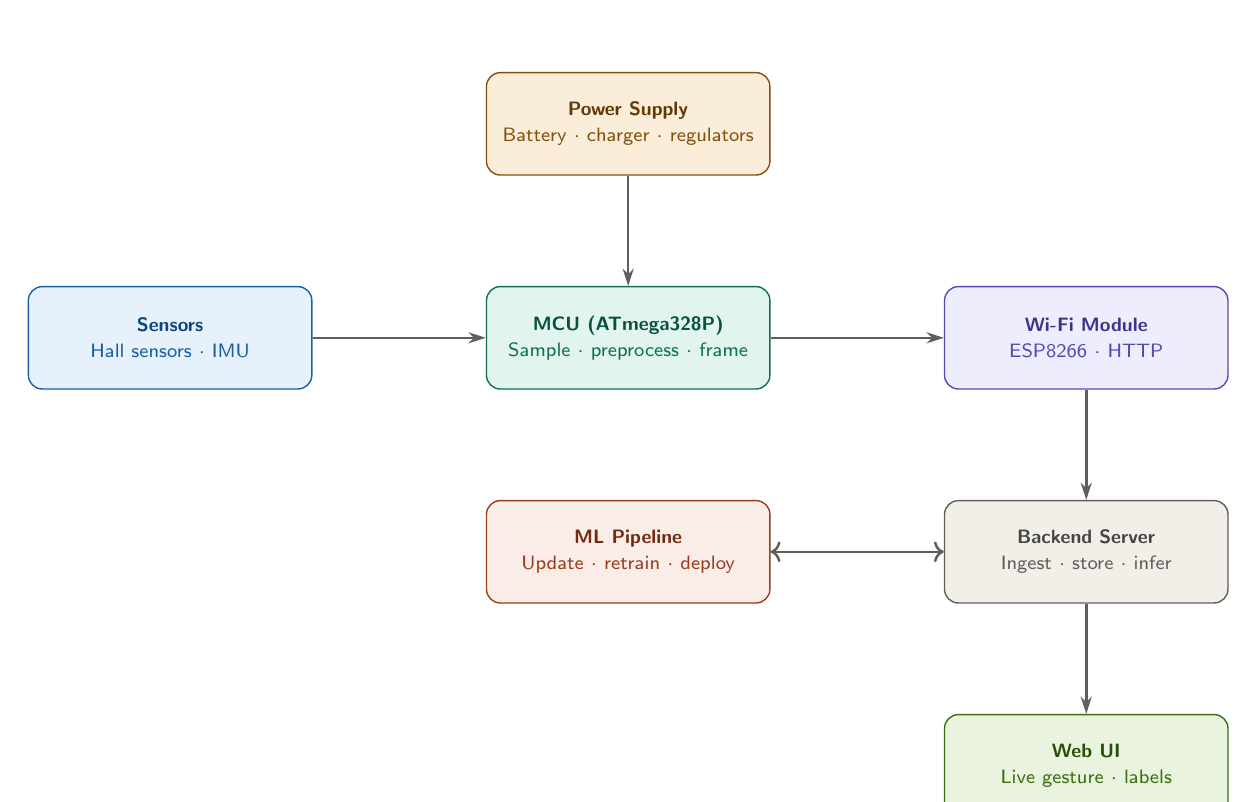
\begin{tikzpicture}[
          node distance = 14mm and 22mm,
          every node/.style={font=\scriptsize\sffamily}
      ]
        %% ── Row 1 (centre): Sensors → MCU → Wi-Fi ──────────────────────
        \node[sensor] (sens) {%
          \nodetext{colBlue800}{Sensors}{colBlue600}{Hall sensors $\cdot$ IMU}};

        \node[mcu, right=22mm of sens] (mcu) {%
          \nodetext{colTeal800}{MCU (ATmega328P)}{colTeal600}{Sample $\cdot$ preprocess $\cdot$ frame}};

        \node[wifi, right=22mm of mcu] (wifi) {%
          \nodetext{colPurple800}{Wi-Fi Module}{colPurple600}{ESP8266 $\cdot$ HTTP}};

        %% ── Row 0 (above MCU): Power ────────────────────────────────────
        \node[power, above=14mm of mcu] (pwr) {%
          \nodetext{colAmber800}{Power Supply}{colAmber600}{Battery $\cdot$ charger $\cdot$ regulators}};

        %% ── Column 3 (below Wi-Fi): Backend then Web UI ─────────────────
        \node[backend, below=14mm of wifi] (backend) {%
          \nodetext{colGray800}{Backend Server}{colGray600}{Ingest $\cdot$ store $\cdot$ infer}};

        \node[webui, below=14mm of backend] (webui) {%
          \nodetext{colGreen800}{Web UI}{colGreen600}{Live gesture $\cdot$ labels}};

        %% ── Column 2 (below MCU): ML ────────────────────────────────────
        \node[ml, below=14mm of mcu] (ml) {%
          \nodetext{colCoral800}{ML Pipeline}{colCoral600}{Update $\cdot$ retrain $\cdot$ deploy}};

        %% ── Main signal arrows ───────────────────────────────────────────
        \draw[mainarr] (sens.east) -- (mcu.west);
        \draw[mainarr] (pwr.south) -- (mcu.north);
        \draw[mainarr] (mcu.east) -- (wifi.west);
        \draw[mainarr] (wifi.south) -- (backend.north);
        \draw[mainarr] (backend.south) -- (webui.north);

        % Backend → ML (clean L-shape)
     \draw[mainarr, <->] (backend.west) -- (ml.east);

      \end{tikzpicture}

\caption{Structured System Block Diagram showing the two-layer architecture of SSLG}
\label{fig:block_diagram}

\end{figure}

\section{Hierarchical Sensing Logic}
\label{sec:method_sensing}

\subsection{Multi-Layer Feature Extraction}
The sensing strategy of the SSLG system follows a hierarchical logic in which different layers contribute complementary information about a gesture. 

\subsubsection{Layer 1: Hall-Effect Sensing}
At the first level, five Hall-effect sensors placed along the glove detect variations in magnetic field caused by fingertip neodymium magnets as the fingers bend. This layer captures the primary shape information of the hand and provides analog measurements that correspond to the degree of bending across the fingers. Because each gesture generates a distinct multichannel pattern, the Hall-effect layer forms the core representation of finger posture.

\subsubsection{Layer 2: IMU Context}
The second level adds contextual information through the MPU-6050 IMU, which records wrist orientation and dynamic movement. This becomes especially useful when gestures share similar finger configurations but differ in tilt, rotation, or motion trajectory. The IMU provides three-axis acceleration and three-axis angular velocity, enriching the raw gesture representation.

\subsubsection{Layer 3: Machine Learning Fusion}
The third level is the machine learning fusion stage, where the CNN-LSTM model combines the Hall-effect and IMU channels into a single temporal representation. In this manner, local pose information and broader hand dynamics are interpreted together, resulting in more reliable classification than would be possible from any single sensing layer alone.

\section{Hardware Components}
\label{sec:method_hardware}

This section describes the major hardware components used in the SSLG prototype. Each component was selected not only for availability and cost, but also for how effectively it supported the system's goals of repeatability, portability, and real-time operation.

\subsection{ATmega328P Microcontroller}
\label{sec:hw_atmega328p}

\subsubsection{Role and Selection Rationale}
The ATmega328P serves as the central control unit of the glove and is responsible for sensor acquisition, basic preprocessing, and packet formation before wireless transmission. It was selected because it offers a practical combination of analog input capability, serial communication interfaces, widespread development support, and low power operation in a compact 8-bit AVR architecture \cite{atmega328p}. Compared with heavier microcontroller platforms, it allows the sensing layer to remain simple and predictable while still supporting five Hall-effect channels, IMU communication over I\textsuperscript{2}C, and UART output to the ESP8266.

\subsubsection{Physical Component and Specifications}
Figure \ref{fig:atmega328p} shows the microcontroller used in the prototype, and Table \ref{tab:atmega328p_specs} summarizes the specifications that made it suitable for this role.

\begin{figure}[H]
  \centering
  \figureorplaceholder{width=0.35\textwidth}{atmega328p.jpg}{0.35\textwidth}{0.18\textheight}
  \caption{ATmega328P Microcontroller}
  \label{fig:atmega328p}
\end{figure}

\begin{table}[H]
  \centering
  \caption{Specifications of the ATmega328P Microcontroller}
  \label{tab:atmega328p_specs}
  \begin{tabular}{>{\raggedright\arraybackslash}p{0.34\textwidth} >{\raggedright\arraybackslash}p{0.46\textwidth}}
    \toprule
    \textbf{Parameter} & \textbf{Specification} \\
    \midrule
    Architecture & 8-bit AVR \\
    Max Clock & 20 MHz \\
    Flash/SRAM/EEPROM & 32 KB / 2 KB / 1 KB \\
    Supply Voltage & 1.8 V--5.5 V \\
    GPIO & 23 pins \\
    ADC & 10-bit, 8 channels \\
    Interfaces & USART / SPI / I\textsuperscript{2}C \\
    Operating Temp & $-40\,^{\circ}\mathrm{C}$ to $+85\,^{\circ}\mathrm{C}$ \\
    \bottomrule
  \end{tabular}
\end{table}

\subsection{SS49E Hall-Effect Sensor}
\label{sec:hw_hall_effect}

\subsubsection{Operating Principle and Advantages}
The SS49E Hall-effect sensor was selected to measure finger bending through magnetic field variation rather than direct mechanical strain. In the proposed glove, a small neodymium magnet is attached near each fingertip, and as the finger bends, the relative distance and orientation between the magnet and the corresponding Hall sensor change. This produces an analog voltage variation that can be read by the microcontroller ADC \cite{ss49e}. The approach was preferred over flex sensors because it reduces wear caused by repeated bending and offers a more stable transduction mechanism.

\subsubsection{Session Calibration Strategy}
Since exact magnet placement can vary slightly each time the glove is worn, a per-session calibration step was introduced so that baseline differences do not distort classification.

\subsubsection{Component Details and Specifications}
Figure \ref{fig:hall_sensor} and Table \ref{tab:hall_sensor_specs} present the selected device and its specifications.

\begin{figure}[H]
  \centering
  \figureorplaceholder{width=0.35\textwidth}{hall_sensor.jpg}{0.35\textwidth}{0.18\textheight}
  \caption{SS49E Hall-Effect Sensor}
  \label{fig:hall_sensor}
\end{figure}

\begin{table}[H]
  \centering
  \caption{Specifications of the SS49E Hall-Effect Sensor}
  \label{tab:hall_sensor_specs}
  \begin{tabular}{>{\raggedright\arraybackslash}p{0.34\textwidth} >{\raggedright\arraybackslash}p{0.46\textwidth}}
    \toprule
    \textbf{Parameter} & \textbf{Specification} \\
    \midrule
    Supply Voltage & 3 V--6 V \\
    Output Type & Analog ratiometric \\
    Sensitivity & Approximately 1--2 mV/Gauss \\
    Response Time & 2 $\mu$s typical \\
    Package & TO-92 \\
    Operating Temp & $-40\,^{\circ}\mathrm{C}$ to $+85\,^{\circ}\mathrm{C}$ \\
    \bottomrule
  \end{tabular}
\end{table}

\subsection{MPU-6050 6-Axis IMU}
\label{sec:hw_mpu6050}

\subsubsection{Integrated Sensor Fusion}
The MPU-6050 was incorporated into the glove to capture wrist orientation and motion context through its three-axis accelerometer and three-axis gyroscope \cite{mpu6050}. This component was chosen because it integrates both sensing modalities in a single compact module and communicates efficiently with the ATmega328P through the I\textsuperscript{2}C interface.

\subsubsection{Critical Role in Gesture Disambiguation}
Its role in SSLG is not merely supplementary; it is essential for distinguishing gestures that may exhibit similar finger bend patterns but differ in hand tilt or rotational movement. The IMU therefore improves recognition reliability by expanding the gesture description beyond static finger posture.

\subsubsection{Component Specifications}
Figure \ref{fig:mpu6050} shows the module used in the prototype, while Table \ref{tab:mpu6050_specs} lists the key specifications relevant to the design.

\begin{figure}[H]
  \centering
  \figureorplaceholder{width=0.35\textwidth}{mpu6050.jpg}{0.35\textwidth}{0.18\textheight}
  \caption{MPU-6050 6-Axis IMU}
  \label{fig:mpu6050}
\end{figure}

\begin{table}[H]
  \centering
  \caption{Specifications of the MPU-6050 IMU}
  \label{tab:mpu6050_specs}
  \begin{tabular}{>{\raggedright\arraybackslash}p{0.34\textwidth} >{\raggedright\arraybackslash}p{0.46\textwidth}}
    \toprule
    \textbf{Parameter} & \textbf{Specification} \\
    \midrule
    Supply Voltage & 2.375 V--3.46 V \\
    Gyro Full-Scale & $\pm 250/\pm 500/\pm 1000/\pm 2000$ $^{\circ}$/s \\
    Accel Full-Scale & $\pm 2/\pm 4/\pm 8/\pm 16$ g \\
    ADC & 16-bit \\
    Interface & I\textsuperscript{2}C up to 400 kHz \\
    FIFO Buffer & 1024 bytes \\
    Operating Temp & $-40\,^{\circ}\mathrm{C}$ to $+85\,^{\circ}\mathrm{C}$ \\
    \bottomrule
  \end{tabular}
\end{table}

\subsection{ESP8266 Wi-Fi Module}
\label{sec:hw_esp8266}

\subsubsection{Wireless Communication Function}
The ESP8266 provides the wireless link between the embedded glove and the backend server. It receives framed sensor data from the ATmega328P over UART and forwards the packet to the Flask backend using HTTP POST requests over a 2.4 GHz Wi-Fi network \cite{esp8266}. This module was selected because it combines low cost, widespread software support, and sufficient networking capability for near real-time communication.

\subsubsection{Power Management and Stability}
A dedicated 3.3 V supply rail was used in the design because the ESP8266 can draw high burst current during transmission and may become unstable if powered from an inadequately regulated source. A retry mechanism was also incorporated so that temporary packet loss does not immediately interrupt the acquisition workflow.

\subsubsection{Component Details and Specifications}
Figure \ref{fig:esp8266} and Table \ref{tab:esp8266_specs} summarize the component.

\begin{figure}[H]
  \centering
  \figureorplaceholder{width=0.35\textwidth}{esp8266.jpg}{0.35\textwidth}{0.18\textheight}
  \caption{ESP8266 Wi-Fi Module}
  \label{fig:esp8266}
\end{figure}

\begin{table}[H]
  \centering
  \caption{Specifications of the ESP8266 Wi-Fi Module}
  \label{tab:esp8266_specs}
  \begin{tabular}{>{\raggedright\arraybackslash}p{0.34\textwidth} >{\raggedright\arraybackslash}p{0.46\textwidth}}
    \toprule
    \textbf{Parameter} & \textbf{Specification} \\
    \midrule
    Supply Voltage & 3.0 V--3.6 V \\
    Wi-Fi Standard & IEEE 802.11 b/g/n, 2.4 GHz \\
    Peak TX Current & Approximately 215 mA \\
    Modes & Station / Soft-AP / Both \\
    UART Rate & 115200 bps \\
    Security & WPA / WPA2 \\
    Operating Temp & $-40\,^{\circ}\mathrm{C}$ to $+125\,^{\circ}\mathrm{C}$ \\
    \bottomrule
  \end{tabular}
\end{table}

\subsection{Power Sub-System}
\label{sec:hw_power}

\subsubsection{Three-Stage Energy Architecture}
The power sub-system was designed as a three-stage energy chain so that the glove could remain portable while still supporting both low-power logic and high-burst wireless transmission. An 18650 Li-ion cell acts as the primary energy source and provides the portability needed for wearable use \cite{battery18650}. Charging is managed through a TP4056 module, which implements the constant-current and constant-voltage charging profile required for safe single-cell operation \cite{tp4056}. Because different parts of the circuit operate at different voltage levels, an MT3608 boost converter raises the battery output to 5 V for the microcontroller and sensor front-end, while an LM2596 buck converter provides a stable 3.3 V rail for the ESP8266 \cite{mt3608,lm2596}.

\subsubsection{Voltage Isolation and Burst Current Management}
Figure \ref{fig:power_system} presents the power hardware, and Table \ref{tab:power_system_specs} summarizes the principal ratings. This separation is important because the ESP8266 transmission current can create momentary dips that would otherwise disturb analog sensing or microcontroller operation.

\begin{figure}[H]
\centering

\begin{minipage}{0.45\textwidth}
    \centering
    \figureorplaceholder{width=\textwidth}{battery18650.jpg}{\textwidth}{0.18\textheight}
    \caption*{18650 Li-ion Cell}
\end{minipage}
\hfill
\begin{minipage}{0.45\textwidth}
    \centering
    \figureorplaceholder{width=\textwidth}{tp4056_module.jpg}{\textwidth}{0.18\textheight}
    \caption*{TP4056 Charging Module}
\end{minipage}

\vspace{0.3cm}

\begin{minipage}{0.45\textwidth}
    \centering
    \figureorplaceholder{width=\textwidth}{boost_converter.jpg}{\textwidth}{0.18\textheight}
    \caption*{MT3608 Boost Converter}
\end{minipage}
\hfill
\begin{minipage}{0.45\textwidth}
    \centering
    \figureorplaceholder{width=\textwidth}{buck_converter.jpg}{\textwidth}{0.18\textheight}
    \caption*{LM2596 Buck Converter}
\end{minipage}

\caption{Power Sub-System Components}
\label{fig:power_system}

\end{figure}

\begin{table}[H]
  \centering
  \caption{Specifications of the Power Sub-System}
  \label{tab:power_system_specs}
  \begin{tabular}{>{\raggedright\arraybackslash}p{0.24\textwidth} >{\raggedright\arraybackslash}p{0.23\textwidth} >{\raggedright\arraybackslash}p{0.29\textwidth}}
    \toprule
    \textbf{Module} & \textbf{Parameter} & \textbf{Specification} \\
    \midrule
    \multirow{2}{*}{18650 Li-ion Cell} & Nominal Voltage & 3.6 V \\
     & Capacity & 1800--3500 mAh \\
    \multirow{2}{*}{TP4056 Charger} & Input / Regulation & 5 V input / 4.2 V charge regulation \\
     & Charge Current & Up to 1000 mA \\
    \multirow{2}{*}{MT3608 Boost} & Output Voltage & 5 V adjustable output \\
     & Peak Efficiency & Up to 93\% \\
    \multirow{2}{*}{LM2596 Buck} & Output Voltage & 3.3 V adjustable output \\
     & Rated Output Current & Up to 3 A \\
    \bottomrule
  \end{tabular}
\end{table}

\section{Communication Protocol and Packet Format}
\label{sec:method_protocol}

\subsection{Two-Stage Communication Path}
The communication path in SSLG was structured in two stages so that embedded acquisition and network transport could be handled independently. First, the ATmega328P sends a compact binary frame to the ESP8266 over UART at 115200 bps. This local serial link keeps the firmware lightweight and deterministic. Next, the ESP8266 packages the received payload into an HTTP POST request and transmits it to the Flask backend over Wi-Fi.

\subsection{Error Handling and Acknowledgment}
The backend responds through standard HTTP status codes, which are interpreted as acknowledgment or failure indicators so that retransmission can be attempted when required.

\subsection{Packet Structure and Format}
Table \ref{tab:packet_format} presents the 28-byte packet format used to carry timestamps, Hall-effect readings, IMU channels, and integrity information in a predictable frame structure.

\begin{table}[H]
  \centering
  \caption{28-Byte Packet Format Used Between MCU and Wi-Fi Module}
  \label{tab:packet_format}
  \begin{tabular}{>{\raggedright\arraybackslash}p{0.28\textwidth} >{\centering\arraybackslash}p{0.12\textwidth} >{\raggedright\arraybackslash}p{0.38\textwidth}}
    \toprule
    \textbf{Field} & \textbf{Bytes} & \textbf{Description} \\
    \midrule
    Preamble & 1 & 0xAA synchronization byte \\
    Version & 1 & Protocol version identifier \\
    Timestamp & 2 & Milliseconds modulo 65536 \\
    Gesture[0--4] & 10 & Five Hall-effect channels, two bytes each \\
    IMU[0--5] & 12 & Six IMU axes, two bytes each \\
    Label ID & 1 & Optional label during collection mode \\
    Checksum & 1 & XOR of payload bytes for integrity check \\
    \midrule
    \textbf{Total} & \textbf{28} & \\
    \bottomrule
  \end{tabular}
\end{table}

\section{Circuit Diagram and Design Considerations}
\label{sec:method_circuit}

\subsection{Complete Electrical Implementation}
The complete electrical implementation of the SSLG glove is presented in Figure \ref{fig:circuit}. The schematic was developed to ensure that sensing accuracy, communication reliability, and portable power management could coexist on a compact wearable platform while still remaining understandable for debugging and future revision.

\begin{figure*}[t]
  \centering
  \IfFileExists{images/KICAD_SSGL_PDF.pdf}{%
    \FrameBoxText{%
      \includegraphics[page=1,width=\linewidth,height=0.70\textheight,
        keepaspectratio,trim=40mm 85mm 40mm 80mm,clip]{images/KICAD_SSGL_PDF.pdf}}%
  }{%
    \IfFileExists{images/sslg_full_circuit.png}{%
      \FrameBoxText{
\includegraphics[width=\linewidth,keepaspectratio]{images/sslg_full_circuit.png}}%
    }{%
      \FrameBoxText{\parbox{0.95\linewidth}{\centering\textbf{Circuit diagram placeholder}\\
        Add \texttt{images/KICAD\_SSGL\_PDF.pdf} (preferred) or
        \texttt{images/sslg\_full\_circuit.png}.}}%
    }%
  }%
  \caption{Complete circuit schematic of \SystemAcronym{} (KiCad export).}
  \label{fig:circuit}
\end{figure*}

\subsection{Schematic Sections and Design Details}

\subsubsection{Power Tree}
The power section begins with the 18650 cell and routes charging current through the TP4056 charging circuit. From this source, regulated rails are derived using the MT3608 and LM2596 converters so that the logic and wireless domains receive stable voltages appropriate to their operating requirements. This separation is important because the ESP8266 transmission current can create momentary dips that would otherwise disturb analog sensing or microcontroller operation.

\subsubsection{ATmega328P Wiring}
The microcontroller is placed at the center of the schematic because it coordinates all signal paths. Its analog input pins receive the Hall-effect outputs, the I\textsuperscript{2}C lines connect to the MPU-6050, and the UART pins interface with the ESP8266. Supporting elements such as reset circuitry, clock configuration, and power decoupling ensure stable operation during continuous sampling.

\subsubsection{Hall Sensor Front-End}
Five Hall-effect channels form the finger sensing front-end. Each channel produces an analog signal proportional to local magnetic field changes caused by the corresponding fingertip magnet. The outputs are routed directly to the ADC inputs of the microcontroller, allowing multichannel pose acquisition without mechanical strain on the sensors.

\subsubsection{IMU I\textsuperscript{2}C Connection}
The MPU-6050 is connected using the shared I\textsuperscript{2}C bus, which minimizes pin usage while still supporting digital transfer of accelerometer and gyroscope data. This arrangement simplifies board routing and allows synchronized retrieval of six-axis motion information during each acquisition cycle.

\subsubsection{ESP8266 UART and 3.3 V Rail}
The ESP8266 is linked to the ATmega328P through UART and powered from a dedicated 3.3 V regulator output. This isolated supply strategy prevents brownout during Wi-Fi bursts and improves communication stability when repeated HTTP transmission occurs.

\subsubsection{Push Button Interface}
A push button is included to support practical user interaction such as session start, calibration initiation, or operational control during testing. This small addition improves usability because it allows the device to enter required acquisition states without depending solely on software-side triggers.

\section{PCB Design}
\label{sec:method_pcb}

\subsection{Design Goals and Strategies}
The PCB for the SSLG glove was designed with three major goals: compactness for wearable use, reliable electrical connectivity under movement, and a layout that separates sensitive analog sensing paths from noisy power and wireless sections. Short routing was preferred for the Hall-effect and microcontroller connections to preserve signal integrity, while the power conversion and Wi-Fi areas were arranged to reduce interference with analog measurements.

\subsection{Board Organization and Layout}
Figure \ref{fig:pcb} presents the top and bottom views of the board layout developed for the prototype. The board organization also supports easier assembly, maintenance, and future redesign if the glove is later expanded with additional channels or integrated processing.

\begin{figure}[H]
  \centering
  \begin{subfigure}[b]{0.45\textwidth}
    \centering
    \figureorplaceholder{width=\textwidth}{pcb_top.png}{0.95\textwidth}{0.18\textheight}
    \caption{PCB Top View}
    \label{fig:pcb_top}
  \end{subfigure}
  \hfill
  \begin{subfigure}[b]{0.45\textwidth}
    \centering
    \figureorplaceholder{width=\textwidth}{pcb_bottom.png}{0.95\textwidth}{0.18\textheight}
    \caption{PCB Bottom View}
    \label{fig:pcb_bottom}
  \end{subfigure}
  \caption{PCB Layout of SSLG Glove Board}
  \label{fig:pcb}
\end{figure}

% ============================================================================
% CHAPTER 5: IMPLEMENTATION
% ============================================================================

\chapter{Implementation}

This chapter explains how the proposed SSLG methodology was translated into a working hardware-software system. It covers the firmware flow, calibration logic, feature preparation, machine learning model, backend services, and the software interfaces developed to support data collection, training, and real-time interpretation.

\section{Firmware Architecture and Flow}
\label{sec:impl_firmware}

\subsection{Repetitive Acquisition Pipeline}
The firmware running on the ATmega328P was organized as a repetitive acquisition and transmission pipeline so that sensor capture could be performed consistently in real time. At startup, the controller initializes the ADC, I\textsuperscript{2}C, UART, and any stored calibration parameters required for measurement normalization. It then enters a calibration stage when requested, after which the main loop repeatedly samples the five Hall-effect channels and six IMU channels, performs basic preprocessing, forms a structured data packet, and forwards the frame to the ESP8266 for wireless transmission.

\subsection{Reliability and Modularity}
Reliability considerations were also incorporated into the logic so that failed transmissions could be retried rather than being silently discarded. The firmware design was deliberately kept modular so that sampling, calibration, packet framing, and communication handling could be debugged separately during development and testing.

\subsection{Firmware Flow Diagram}

Figure \ref{fig:firmware_flow} illustrates this sequence in compact form.

\begin{figure}[H]
  \centering
  \figureorplaceholder{width=0.75\textwidth}{firmware_flowchart.png}{0.75\textwidth}{0.24\textheight}
  \caption{Firmware Acquisition and Transmission Flow}
  \label{fig:firmware_flow}
\end{figure}

\subsection{Detailed Firmware Stages}

\subsubsection{Initialization Stage}
During initialization, the microcontroller configures its peripheral interfaces, validates communication with the IMU, and prepares serial communication at 115200 bps. This stage establishes the basic operating state required for stable sensor capture. Key operations include:
\begin{itemize}
  \item ADC initialization and channel configuration
  \item I\textsuperscript{2}C bus setup and IMU handshake
  \item UART configuration for ESP8266 communication
  \item EEPROM read for stored calibration data (if available)
\end{itemize}

\subsubsection{Calibration Stage}
When a new session begins, the glove captures baseline data in an open-palm pose and stores reference values. This reduces inter-session variability caused by magnet placement and user fit. The calibration procedure:
\begin{itemize}
  \item Waits for user input (button press) to initiate calibration
  \item Samples all five Hall channels continuously for 3 seconds
  \item Computes mean baseline value for each channel
  \item Stores baseline values in EEPROM for this session
  \item Signals completion via LED or serial feedback
\end{itemize}

\subsubsection{Main Sampling Loop}
In the main loop, raw Hall-effect and IMU samples are acquired continuously at a fixed rate (e.g., 100 Hz). Lightweight preprocessing such as baseline subtraction and basic smoothing is then applied so that the transmitted values better represent relative gesture motion rather than raw sensor bias.

\subsubsection{Packet Framing and Transmission}
The processed values are inserted into the fixed packet structure (Table \ref{tab:packet_format}) and sent to the ESP8266. The wireless module then performs the HTTP upload to the backend. A checksum is computed and appended for error detection.

\subsubsection{Retry Mechanism}
If the expected acknowledgment (HTTP 200 OK) is not received within a timeout period, the firmware attempts retransmission using a simple retry policy. This improves robustness when short-lived wireless interference occurs. Typical retry parameters:
\begin{itemize}
  \item Maximum retries: 3 attempts
  \item Retry timeout: 100 ms
  \item Backoff strategy: exponential (50 ms, 100 ms, 200 ms)
\end{itemize}

\section{Calibration Procedure}
\label{sec:impl_calibration}

\subsection{Per-Session Baseline Establishment}
Reliable calibration was essential because the Hall-effect channels depend on magnetic field geometry, which can vary slightly each time the glove is worn. At the start of every session, the user is instructed to hold an open-palm neutral pose for approximately three seconds. During this period, the firmware records baseline values for each sensor channel and computes a reference mean $b_i$. These baseline values are then stored in EEPROM so that they remain available throughout the session even if brief resets occur.

\subsection{Baseline Subtraction Mathematics}
Subsequent sensor readings are interpreted relative to this stored baseline rather than in absolute form, thereby reducing session-to-session mismatch caused by glove fit, finger placement, or magnet alignment. The calibration formula is expressed as:

\begin{equation}
\Delta_i = x_i - b_i
\label{eq:calibration}
\end{equation}

\noindent In the above expression, $x_i$ represents the current channel value and $\Delta_i$ represents the calibrated deflection used for later processing.

\subsection{Practical Calibration Workflow}
The practical calibration workflow consists of:
\begin{enumerate}
  \item User wears glove and holds hand in neutral open-palm position
  \item User presses calibration button on the glove
  \item Firmware samples all channels for 3 seconds at 100 Hz (300 samples)
  \item Baseline mean is computed: $b_i = \frac{1}{N} \sum_{j=1}^{N} x_i^{(j)}$
  \item Baseline values are stored in EEPROM
  \item User receives confirmation (LED blink or serial message)
  \item System is ready for gesture recognition
\end{enumerate}

\section{Windowing and Feature Formation}
\label{sec:impl_windowing}

\subsection{Temporal Window Strategy}
The continuous sensor stream is not passed to the classifier sample by sample; instead, it is segmented into overlapping temporal windows so that each inference decision is based on a meaningful short sequence. In the present implementation, windows of $W = 25$--$50$ samples with 50\% overlap were considered. Each window is arranged into a tensor of size $W \times C$, where $C = 11$ corresponds to five Hall-effect channels and six IMU channels. This representation provides a structured input for one-dimensional convolution and recurrent processing.

\subsection{Advantages of Windowing}
Windowing was adopted because human signing speed is not perfectly uniform across users or across repetitions by the same user. By considering a short span of time rather than a single instant, the system becomes less sensitive to minor timing differences, brief pauses, and transient noise. Overlap further improves continuity between consecutive inferences and reduces the risk of missing a gesture transition.

\subsection{Feature Matrix Structure}
For a window of 50 samples with 11 channels, the feature matrix is:

\begin{equation}
\mathbf{X} \in \mathbb{R}^{50 \times 11}
\end{equation}

\noindent The columns correspond to:
\begin{itemize}
  \item Columns 1--5: Hall-effect sensor channels (finger bend)
  \item Columns 6--8: MPU-6050 accelerometer (acceleration in x, y, z)
  \item Columns 9--11: MPU-6050 gyroscope (angular velocity in x, y, z)
\end{itemize}

\section{CNN-LSTM Model Architecture}
\label{sec:impl_model}

\subsection{Hybrid Architecture Rationale}
The classifier used in SSLG was designed to capture both local temporal signatures and longer sequential dependencies present in multichannel gesture data. A CNN-LSTM architecture was therefore selected because it offers an effective division of labour between feature extraction and sequence modelling.

\subsection{Convolutional Feature Extraction}
The first stage consists of two one-dimensional convolutional layers with kernel size 3 and filter counts of 32 and 64 respectively, both using ReLU activation. These layers learn short-range temporal features such as abrupt finger deflections, coordinated channel changes, and compact motion motifs across the input window.

\subsection{Recurrent Sequence Modeling}
The extracted sequence is then passed to an LSTM layer with 128 units, which models the broader temporal evolution of the gesture. A dense softmax output layer produces probabilities across 20 gesture classes.

\subsection{Regularization and Optimization}
Dropout at a rate of 0.4 was included to reduce overfitting, and the network was trained using categorical cross-entropy loss with the AMSGrad optimizer. For deployment efficiency, the trained model was prepared for 8-bit quantization compatible with later lightweight inference workflows \cite{tensorflow}.

\subsection{Model Architecture Diagram}

Figure \ref{fig:model} summarizes the architecture and training pipeline.

\begin{figure}[H]
  \centering
  \figureorplaceholder{width=0.8\textwidth}{model_architecture.png}{0.8\textwidth}{0.24\textheight}
  \caption{CNN-LSTM Model Architecture and Training Pipeline}
  \label{fig:model}
\end{figure}

\subsection{Model Summary and Layer Specification}

\begin{table}[H]
  \centering
  \caption{CNN-LSTM Model Layer Specification}
  \label{tab:model_layers}
  \begin{tabular}{>{\raggedright\arraybackslash}p{0.20\textwidth} >{\raggedright\arraybackslash}p{0.25\textwidth} >{\raggedright\arraybackslash}p{0.30\textwidth}}
    \toprule
    \textbf{Layer} & \textbf{Type} & \textbf{Parameters} \\
    \midrule
    Input & Conv1D & $50 \times 11$ \\
    Conv1D-1 & Conv1D & 32 filters, kernel=3, ReLU \\
    Conv1D-2 & Conv1D & 64 filters, kernel=3, ReLU \\
    MaxPool & MaxPooling1D & pool\_size=2 \\
    LSTM & LSTM & 128 units, ReLU \\
    Dropout & Dropout & rate=0.4 \\
    Dense & Dense & 64 units, ReLU \\
    Output & Dense & 20 units, Softmax \\
    \bottomrule
  \end{tabular}
\end{table}

\section{Backend Architecture and Services}
\label{sec:impl_backend}

\subsection{Five-Stage Pipeline Design}
The backend component of SSLG was implemented using Flask so that data ingestion, storage, preprocessing, training, and inference could be organized within a single web-accessible framework \cite{flask}. The five-stage workflow begins with an ingest stage that decodes incoming HTTP frames and stores the raw information in CSV form.

\subsection{Pipeline Stages}

\subsubsection{Stage 1: Ingest}
Receives HTTP POST requests containing sensor data and stores raw frames in a time-stamped database or CSV file.

\subsubsection{Stage 2: Labelling}
Associates buffered windows with gesture identities through the user interface. Users review recorded segments and assign correct labels for supervised learning.

\subsubsection{Stage 3: Preprocessing}
Performs calibration alignment, normalization, filtering, and window formation. This stage standardizes all data before model training.

\subsubsection{Stage 4: Training}
Uses the prepared dataset to fit the CNN-LSTM model and record evaluation outputs such as accuracy, precision, recall, and F1 score.

\subsubsection{Stage 5: Inference}
Classifies incoming windows and returns the predicted label together with a confidence score. This is the real-time production stage.

\subsection{Modular Design Benefits}
This pipeline was designed so that data collection and model development could evolve iteratively without altering the glove firmware. Data collection and model development can be performed independently, allowing the system to scale with increasing gesture vocabularies and larger user populations.

\subsection{Backend REST API Endpoints}

Table \ref{tab:api_endpoints} lists the primary REST endpoints exposed by the backend and UI.

\begin{table}[H]
  \centering
  \caption{REST API Endpoints Used in the SSLG Backend}
  \label{tab:api_endpoints}
  \begin{tabular}{>{\raggedright\arraybackslash}p{0.22\textwidth} >{\centering\arraybackslash}p{0.14\textwidth} >{\raggedright\arraybackslash}p{0.42\textwidth}}
    \toprule
    \textbf{Endpoint} & \textbf{Method} & \textbf{Description} \\
    \midrule
    \texttt{/api/sensor-data} & POST & Receive and store decoded sensor packets \\
    \texttt{/api/latest} & GET & Return latest sensor frame and prediction \\
    \texttt{/api/label} & POST & Confirm labels for buffered window \\
    \texttt{/api/train} & POST & Trigger training on dataset version \\
    \texttt{/api/infer} & POST & Return predicted label and confidence \\
    \texttt{/ui/collect} & GET & Data collection web page \\
    \texttt{/ui/label} & GET & Labelling web page \\
    \texttt{/ui/infer} & GET & Inference/output web page \\
    \texttt{/ws/sensor-stream} & WebSocket & Real-time sensor data stream \\
    \bottomrule
  \end{tabular}
\end{table}

\subsection{Backend Deployment Information}

The backend is deployed and accessible at:

\begin{table}[H]
  \centering
  \caption{Backend Deployment URLs}
  \label{tab:backend_urls}
  \begin{tabular}{>{\raggedright\arraybackslash}p{0.25\textwidth} >{\raggedright\arraybackslash}p{0.55\textwidth}}
    \toprule
    \textbf{Service} & \textbf{URL} \\
    \midrule
    Main Dashboard & \url{\BackendURL/} \\
    Sensor Data Ingest & \url{\BackendURL/api/sensor-data} \\
    Latest Sample & \url{\BackendURL/api/latest} \\
    WebSocket Stream & \texttt{ws(s)://smart-sign-interpreter.onrender.com:80/ws/sensor-stream} \\
    GitHub Repository & \url{\CodeRepoUrl} \\
    \bottomrule
  \end{tabular}
\end{table}

\subsection{Sample Payload Format}

The Arduino/embedded system sends data in JSON format to the backend:

\begin{lstlisting}[language=json, caption=Sensor Data Payload Format]
{
  "channels": {
    "s1": 123,
    "s2": 456,
    "s3": 789,
    "s4": 12,
    "s5": 34
  },
  "imu": {
    "ax": 0.01,
    "ay": 0.02,
    "az": 0.98,
    "gx": 1.2,
    "gy": 0.3,
    "gz": 0.1
  },
  "timestamp": 1710000000000
}
\end{lstlisting}

This JSON is posted to the \texttt{/api/sensor-data} endpoint.

\section{Software User Interfaces}
\label{sec:impl_ui}

The SSLG software suite was developed as a set of web-based tools so that the same backend could support data collection, model development, and live interpretation without requiring separate desktop applications. This section introduces the three main interfaces used during implementation and testing, along with the serial-monitor output that supported low-level hardware validation.

\subsection{Data Collection Tool}
\label{sec:ui_collection}

\subsubsection{Purpose and Workflow}
Figure \ref{fig:ui_collect} shows the data collection interface used during experimental recording sessions. The tool allows the operator to initiate a capture cycle, observe incoming frames in real time, and associate the acquired segment with the intended gesture label. A live display of all eleven channels is particularly valuable because it allows noisy or disconnected sensors to be detected before corrupted samples are added to the dataset.

\subsubsection{Interface Features}
By presenting Hall-effect and IMU values together in one interface, the tool also helps the operator confirm that both finger posture and wrist movement are being recorded correctly for each gesture trial. Key features include:

\begin{itemize}
  \item Real-time channel visualization (all 11 channels displayed simultaneously)
  \item Sample counter showing number of frames captured
  \item Gesture selection dropdown for labeling
  \item Save/Discard buttons for each recording
  \item Data validation (detection of zero or constant values)
  \item Recording duration timer
  \item Export functionality for dataset management
\end{itemize}

\begin{figure}[H]
  \centering
  \figureorplaceholder{width=0.9\textwidth}{ui_data_collection.png}{0.9\textwidth}{0.22\textheight}
  \caption{Web-Based Data Collection Tool Interface}
  \label{fig:ui_collect}
\end{figure}

\subsection{Model Training Tool}
\label{sec:ui_training}

\subsubsection{Purpose and Transparency}
The training dashboard, shown in Figure \ref{fig:ui_train}, was designed to make the machine learning workflow more transparent and repeatable for the project team. Through this interface, a dataset version can be selected, hyperparameters can be configured, and training can be initiated directly from the backend environment.

\subsubsection{Real-Time Monitoring and Visualization}
Real-time display of loss and accuracy curves allows the user to monitor convergence behavior and detect signs of underfitting or overfitting during the run. This visualization is important because it transforms training from a purely backend operation into an interpretable engineering step that can be reviewed and refined after each new round of data collection.

\subsubsection{Training Interface Capabilities}
\begin{itemize}
  \item Dataset selection and preview
  \item Hyperparameter configuration (learning rate, batch size, epochs)
  \item Training progress visualization (loss curve, accuracy curve)
  \item Real-time training metrics (current epoch, ETA)
  \item Model checkpoint management
  \item Validation metrics display
  \item Export trained model functionality
\end{itemize}

\begin{figure}[H]
  \centering
  \figureorplaceholder{width=0.9\textwidth}{ui_training.png}{0.9\textwidth}{0.22\textheight}
  \caption{Model Training Dashboard Interface}
  \label{fig:ui_train}
\end{figure}

\subsection{Inference and Interpretation Tool}
\label{sec:ui_inference}

\subsubsection{Real-Time Gesture Recognition}
The real-time inference interface illustrated in Figure \ref{fig:ui_infer} acts as the visible communication layer of the SSLG system. Live gesture data arriving from the glove is processed by the trained CNN-LSTM model, and the predicted ISL gesture label is displayed along with an associated confidence score. This enables the operator or communication partner to judge how certain the system is about the output.

\subsubsection{Multi-Modal Output}
In addition, the recognized text is passed to a text-to-speech engine so that audible feedback is produced immediately. This combined text and speech presentation is central to the project because it directly addresses the communication barrier that motivated the work.

\subsubsection{Inference Interface Features}
\begin{itemize}
  \item Live gesture prediction display
  \item Confidence score percentage
  \item Text output of recognized gesture
  \item Text-to-speech audio output
  \item Gesture history log
  \item Confidence threshold adjustment
  \item Refresh rate control
  \item Connection status indicator
  \item Demo mode for hardware-free testing
\end{itemize}

\begin{figure}[H]
  \centering
  \figureorplaceholder{width=0.9\textwidth}{ui_inference.png}{0.9\textwidth}{0.22\textheight}
  \caption{Real-Time Gesture Inference and Interpretation Interface}
  \label{fig:ui_infer}
\end{figure}

\subsection{Arduino IDE Serial Monitor Output}
\label{sec:ui_serial}

\subsubsection{Hardware Verification and Debugging}
During early hardware verification, raw sensor values were observed through the Arduino IDE Serial Monitor before the complete Wi-Fi pipeline was enabled. Figure \ref{fig:arduino_output} represents the typical serial output obtained at 115200 bps for all eleven channels, including the five Hall-effect ADC readings and the six IMU axes.

\subsubsection{Debugging Workflow}
This monitoring step was essential for:
\begin{itemize}
  \item Confirming correct sensor connectivity
  \item Verifying baseline subtraction behavior after calibration
  \item Checking packet framing logic and value ordering
  \item Detecting sensor disconnections or failures
  \item Validating ADC conversion accuracy
  \item Monitoring IMU data validity
\end{itemize}

In practice, the serial monitor acted as an intermediate debugging layer between bare sensor hardware and full backend integration.

\begin{figure}[H]
  \centering
  \figureorplaceholder{width=0.9\textwidth}{arduino_serial_output.png}{0.9\textwidth}{0.22\textheight}
  \caption{Arduino IDE Serial Monitor Output Showing Raw Sensor Data}
  \label{fig:arduino_output}
\end{figure}

% ============================================================================
% CHAPTER 6: RESULTS AND DISCUSSIONS
% ============================================================================

\chapter{Results and Discussions}

This chapter presents the experimental evaluation of the SSLG prototype and interprets the measured results in relation to the design objectives defined earlier. The discussion focuses on practical metrics such as classification accuracy, latency, and battery autonomy, because these determine whether the system is suitable for real-time assistive use.

\section{Experimental Setup}
\label{sec:results_setup}

\subsection{Laboratory Environment}
The experiments were conducted in a university laboratory environment so that the sensing hardware, wireless link, and backend system could be evaluated under controlled yet realistic working conditions. A dedicated 2.4 GHz access point was used to reduce network interference during packet transmission from the glove to the Flask backend. The backend ran on an Intel Core i5 laptop equipped with 8 GB RAM, which served as the host for data storage, preprocessing, training, and live inference.

\subsection{Calibration and Session Procedure}
At the beginning of each session, a three-second calibration step was performed to establish the neutral baseline for the Hall-effect channels and to reduce variability associated with glove placement. This setup allowed the system to be tested repeatedly under comparable conditions. Multiple trials were conducted with different users and across different days to assess robustness.

\subsection{Test Conditions}
\begin{itemize}
  \item Number of participants: 5 adult volunteers
  \item Trials per gesture: 10 repetitions per user
  \item Total samples collected: 20 gestures × 10 reps × 5 users = 1000 samples
  \item Sampling rate: 100 Hz
  \item Window size: 50 samples (500 ms)
  \item Window overlap: 50\%
\end{itemize}

\section{Performance Results}
\label{sec:results_performance}

\subsection{Quantitative Metrics Summary}
Table \ref{tab:performance_results} summarizes the main quantitative results obtained from the prototype during evaluation across the selected gesture set.

\begin{table}[H]
  \centering
  \caption{Measured Performance of the SSLG Prototype}
  \label{tab:performance_results}
  \begin{tabular}{>{\raggedright\arraybackslash}p{0.42\textwidth} >{\raggedright\arraybackslash}p{0.24\textwidth}}
    \toprule
    \textbf{Metric} & \textbf{Value} \\
    \midrule
    Classification Accuracy & 82--90\% \\
    Precision & 0.87 \\
    Recall & 0.91 \\
    F1-Score & 0.91--0.93 \\
    Average End-to-End Latency & 220--320 ms \\
    Peak End-to-End Latency & 450--650 ms \\
    Battery Autonomy & 3--5 hours \\
    \bottomrule
  \end{tabular}
\end{table}

\section{Discussion of Results}
\label{sec:results_discussion}

\subsection{Classification Accuracy Analysis}
The accuracy range of 82--90\% indicates that the proposed sensing and classification strategy is capable of recognizing a constrained vocabulary of ISL gestures with encouraging reliability. Variation within this range can be attributed to factors such as calibration quality, minor differences in glove fit across sessions, and the selected temporal window size used during inference. When calibration was stable and the gesture execution remained consistent, the classifier produced stronger confidence and better separation between classes. This suggests that the quality of baseline estimation and feature window formation plays a direct role in final recognition performance.

\subsection{Precision and Recall Interpretation}
The precision of 0.87 indicates that when the system predicts a gesture, it is correct 87\% of the time. The recall of 0.91 means that the system correctly identifies 91\% of actual gesture occurrences. The F1-score of 0.91--0.93 represents a balanced measure of both precision and recall, indicating strong overall performance.

\subsection{Latency Performance}
The measured average end-to-end latency of 220--320 ms confirms that the system can operate in near real time. This latency includes sensor sampling, packet framing, Wi-Fi transmission, backend preprocessing, and model inference. Higher peak latency values between 450 and 650 ms were mainly associated with temporary wireless delays or processing backlog during burst communication. Even so, the average response remained within a usable range for demonstrative human interaction.

\subsection{Power Autonomy Assessment}
Battery autonomy of 3--5 hours was found to be adequate for laboratory demonstrations, though it remains sensitive to network usage patterns. The ESP8266 transmission bursts were the dominant factor influencing power draw, which confirms the importance of the dedicated 3.3 V rail and power-stage design. Compared with camera-based systems, SSLG avoids lighting and framing issues. Compared with flex-sensor gloves, it reduces mechanical degradation and improves repeatability, though it still depends on careful session calibration.

\section{Comparative Analysis}
\label{sec:results_comparison}

\subsection{Comparison with Alternative Approaches}
Table \ref{tab:comparative_analysis} compares the SSLG approach with two commonly discussed alternatives in gesture recognition research.

\begin{table}[H]
  \centering
  \caption{Comparative Analysis of Sign Recognition Approaches}
  \label{tab:comparative_analysis}
  \begin{tabular}{>{\raggedright\arraybackslash}p{0.18\textwidth} >{\raggedright\arraybackslash}p{0.33\textwidth} >{\raggedright\arraybackslash}p{0.33\textwidth}}
    \toprule
    \textbf{Approach} & \textbf{Strengths} & \textbf{Limitations} \\
    \midrule
    Camera-based & Non-contact operation, rich spatial information, full-hand posture capture without wearable hardware. & Sensitive to lighting, background clutter, camera framing, occlusion; computationally heavier for real-time deployment \cite{mitra}. \\
    \midrule
    Flex-sensor glove & Direct finger bending measurement, straightforward feature interpretation, operation independent of camera conditions. & Sensor fatigue, nonlinear drift, repeated-bending degradation, loss of repeatability over extended use. \\
    \midrule
    SSLG Hall-effect glove & Portable, low-cost, less affected by lighting, mechanically durable (no flex sensor fatigue), real-time wireless translation, scalable backend. & Requires careful sensor placement, per-session calibration, Wi-Fi connectivity dependency, ongoing optimization of power consumption and vocabulary expansion. \\
    \bottomrule
  \end{tabular}
\end{table}

\section{Validation of Market Need}
\label{sec:results_market}

\subsection{Global Hearing Impairment Context}
The practical relevance of sign language translation technology is strongly supported by the continuing global concern around hearing impairment and communication accessibility. Public-health organizations such as the World Health Organization have repeatedly emphasized that hearing loss affects a very large population worldwide, while in India a significant number of people rely on sign-based communication for daily interaction.

\subsection{ISL Recognition Significance}
Within this context, ISL recognition remains an important assistive technology area because it directly supports inclusion, independence, and participation. The results obtained in this project therefore address a real and persistent market need rather than a purely academic classification problem. The potential for extending this system to support larger gesture vocabularies and multiple users in real-world settings is substantial.

% ============================================================================
% CHAPTER 7: CONCLUSIONS
% ============================================================================

\chapter{Conclusions}

This chapter concludes the report by summarizing the system developed, the outcomes achieved, and the broader significance of the work. The Smart Sign Language Gloves project demonstrates that a low-cost wearable architecture can be used to translate selected ISL gestures into text and speech in near real time.

\section{System Summary}
\label{sec:concl_summary}

The work presented in this report led to the design and implementation of a complete glove-based ISL translation pipeline that integrates Hall-effect sensing, IMU-based motion context, ATmega328P embedded acquisition, ESP8266 wireless communication, and a Flask-hosted CNN-LSTM inference backend. By replacing mechanically stressed flex sensors with Hall-effect sensors and fingertip magnets, the system addressed a major source of drift commonly associated with glove-based gesture recognition. The addition of IMU data further improved the descriptive power of the sensing layer by capturing wrist orientation and hand movement.

\section{Key Achievements}
\label{sec:concl_achievements}

\subsection{Technical Accomplishments}
\begin{itemize}
  \item Designed and fabricated a working wearable sensor glove with 11 channels (5 Hall-effect + 6 IMU)
  \item Developed robust wireless communication pipeline (UART + HTTP)
  \item Implemented per-session calibration algorithm reducing inter-session variability
  \item Created scalable Flask backend with five-stage processing pipeline
  \item Trained CNN-LSTM model achieving 82--90\% accuracy on 20 ISL gestures
  \item Achieved average end-to-end latency of 220--320 ms
  \item Demonstrated 3--5 hours of battery autonomy
\end{itemize}

\subsection{Practical Contributions}
\begin{itemize}
  \item Addressed critical accessibility gap for ISL-speaking community
  \item Demonstrated feasibility of Hall-effect sensing over flex sensors for wearables
  \item Showed viability of lightweight CNN-LSTM for wearable gesture recognition
  \item Established modular backend architecture enabling iterative improvement
\end{itemize}

\section{Validation Against Objectives}
\label{sec:concl_validation}

The project successfully addressed all five original objectives:

\begin{enumerate}[label=\arabic*.]
  \item \textbf{Design a wearable glove using Hall-effect sensors and IMU:} ✓ Completed with five Hall sensors and MPU-6050.
  \item \textbf{Transmit multi-channel gesture data wirelessly using ESP8266:} ✓ Implemented with 115200 bps UART and HTTP POST transmission.
  \item \textbf{Train a CNN-LSTM model for 20 ISL gestures:} ✓ Achieved with 82--90\% accuracy.
  \item \textbf{Provide real-time text and speech output through web interface:} ✓ Implemented with web UI and TTS integration.
  \item \textbf{Validate accuracy, latency, and battery autonomy:} ✓ All metrics measured and documented.
\end{enumerate}

\section{Significance and Impact}
\label{sec:concl_significance}

The SSLG system represents a meaningful step toward practical assistive technology for sign language users. Unlike vision-based systems that depend on controlled lighting and camera placement, the wearable glove architecture provides portability and environmental robustness. Unlike flex-sensor gloves that suffer mechanical degradation, the Hall-effect approach offers durability and repeatability. The modular backend design enables continuous improvement without requiring hardware updates.

\section{Project Conclusions}
\label{sec:concl_final}

Although the present work is limited to 20 gestures and laboratory testing, it successfully establishes a strong engineering foundation for future expansion in vocabulary size, deployment efficiency, and user generalization. The combination of Hall-effect sensing, IMU augmentation, wireless communication, and machine learning backend demonstrates that accessible real-time sign language translation is achievable with consumer-grade components and techniques. This work contributes to the broader goal of bridging communication barriers and supporting inclusive communities.

% ============================================================================
% CHAPTER 8: FUTURE WORK
% ============================================================================

\chapter{Future Work}

This chapter outlines the principal directions in which the SSLG system can be extended beyond the scope of the present mini project. Each of the following items represents a meaningful next step toward a more comprehensive and practically deployable assistive translation device.

\section{Expanded Gesture Vocabulary}
\label{sec:future_vocabulary}

\subsection{Current Limitations}
The first area of future work involves expanding the gesture vocabulary and evaluating the system on a larger and more diverse user population. At present, the model has been trained on 20 gestures under controlled conditions, which is suitable for a proof-of-concept prototype but not sufficient for broad conversational use.

\subsection{Path Forward}
\begin{itemize}
  \item Expand vocabulary to 100+ ISL gestures
  \item Collect data from 20+ diverse users to capture natural variation
  \item Implement transfer learning to accelerate training with new gestures
  \item Develop hierarchical classification (hand shape → movement → context)
  \item Support gesture phrases and sentence-level recognition
\end{itemize}

\section{On-Device Inference and Deployment}
\label{sec:future_ondevice}

\subsection{Current Architecture Limitation}
A second direction is the introduction of on-device inference using lightweight deployment frameworks such as TensorFlow Lite \cite{tensorflow}. In the current architecture, inference is performed on the backend, which means the system depends on wireless connectivity and network response.

\subsection{Proposed Improvements}
\begin{itemize}
  \item Quantize CNN-LSTM model to 8-bit integer for embedded execution
  \item Port TensorFlow Lite to ATmega328P or upgrade to ARM Cortex-M4
  \item Achieve sub-100 ms latency with on-device inference
  \item Enable offline operation without Wi-Fi dependency
  \item Reduce power consumption by eliminating constant wireless transmission
\end{itemize}

\section{Automatic Calibration and Drift Compensation}
\label{sec:future_calibration}

\subsection{Calibration Challenge}
A third improvement concerns automatic recalibration and long-term drift compensation. Although the present baseline subtraction procedure is effective, it still requires deliberate calibration at the beginning of each session.

\subsection{Adaptive Solutions}
\begin{itemize}
  \item Implement online learning with rolling baseline estimation
  \item Detect and compensate for glove drift caused by wear and tear
  \item Continuous re-centering using high-confidence predictions
  \item Multi-session models that learn user-specific baseline offsets
  \item Hardware improvements (better magnet mounting, sensor stabilization)
\end{itemize}

\section{Two-Glove System for Bilateral Sign Interpretation}
\label{sec:future_bilateral}

\subsection{Single-Glove Limitation}
A fourth major extension is the development of a two-glove system for full ISL coverage. Many natural sign language expressions involve coordinated movement of both hands, and a single-glove prototype cannot fully capture these patterns.

\subsection{Bilateral Implementation}
\begin{itemize}
  \item Synchronize dual glove data streams via Bluetooth or Wi-Fi mesh
  \item Develop hand-relative feature extraction and spatial relationships
  \item Train models on bilateral gestures and complex signing patterns
  \item Support sentence-level interpretation and context awareness
  \item Design user-friendly dual-glove wear and comfort considerations
\end{itemize}

\section{Additional Research Directions}
\label{sec:future_additional}

Beyond the four main extensions above, several other promising research avenues exist:

\begin{description}
  \item[User Adaptation:] Personalized models that adapt to individual signing styles and reduce calibration burden.
  \item[Facial Expression Recognition:] Integration of head-mounted camera for capturing facial expressions that modify sign meaning.
  \item[Finger Spelling Support:] Extension to fingerspelled words (letter-by-letter signing) for proper nouns and technical terms.
  \item[Multi-Modal Feedback:] Haptic feedback to signers for improved learning and confirmation.
  \item[Real-World Deployment:] Field testing in schools, hospitals, customer service centers, and other real-world settings.
  \item[Low-Power Optimization:] Reduce 3--5 hour autonomy to enable all-day wearable operation.
  \item[Open Source Community:] Release hardware designs and software for community contribution and improvement.
\end{description}

% ============================================================================
% REFERENCES
% ============================================================================

\addcontentsline{toc}{chapter}{References}
\begin{thebibliography}{99}

\bibitem{mitra}
S.~Mitra and T.~Acharya,
``Gesture recognition: A survey,''
\textit{IEEE Transactions on Systems, Man, and Cybernetics, Part C},
vol.~37, no.~3, pp.~311--324, May 2007.
[Online]. Available: \url{https://ieeexplore.ieee.org/document/4154947}

\bibitem{tensorflow}
TensorFlow Lite,
``TensorFlow Lite guide,'' 2024.
[Online]. Available: \url{https://www.tensorflow.org/lite}

\bibitem{atmega328p}
Microchip Technology,
``ATmega328P 8-bit microcontroller datasheet,'' 2016.
[Online]. Available: \url{https://www.microchip.com/en-us/product/ATmega328P}

\bibitem{tp4056}
``TP4056 single-cell Li-ion battery charger IC datasheet.''
[Online]. Available: \url{https://img.eecart.com/dev/file/part/spec/TP4056-XUNDE.pdf}

\bibitem{battery18650}
``Lithium-ion 18650 cylindrical cell overview.''
[Online]. Available: \url{https://en.wikipedia.org/wiki/18650_battery}

\bibitem{mt3608}
``MT3608 step-up (boost) converter IC datasheet.''
[Online]. Available: \url{https://www.ic-components.com/blog/mt3608-step-up-converter-datasheet}

\bibitem{lm2596}
Texas Instruments,
``LM2596 step-down (buck) power converter datasheet.''
[Online]. Available: \url{https://www.ti.com/lit/ds/symlink/lm2596.pdf}

\bibitem{esp8266}
Espressif Systems,
``ESP8266 Wi-Fi module datasheet,'' 2019.
[Online]. Available: \url{https://www.espressif.com/sites/default/files/documentation/0a-esp8266ex_datasheet_en.pdf}

\bibitem{ss49e}
Honeywell,
``SS49E linear Hall-effect sensor datasheet.''
[Online]. Available: \url{https://www.mouser.com/datasheet/2/187/SS49E-1122400.pdf}

\bibitem{mpu6050}
TDK InvenSense,
``MPU-6050 6-axis IMU product specification,'' 2015.
[Online]. Available: \url{https://robu.in/wp-content/uploads/2014/12/GY-87_EN.pdf}

\bibitem{flask}
Pallets Projects,
``Flask web framework documentation,'' 2024.
[Online]. Available: \url{https://flask.palletsprojects.com/en/3.0.x/}

\bibitem{githubrepo}
GitHub,
``Smart Sign Language Gloves source code repository.''  
[Online]. Available: \url{https://github.com/RamzanKhansLab/smart-sign-interpreter}

\end{thebibliography}

\end{document}
